\section{Sauvegarde}\label{SauvegardeTechnique}
\label{Architecture_technique_de_sauvegarde}

\subsection{Problématique}
La suite logicielle permet de synchroniser des données, à la fois entre postes clients et serveur local, mais également entre serveur local et serveur central, et ce, via les différentes architectures ci dessous.

\subsection{Cluster}
Une première solution utilisant la technologie du \emph{cluster} peut être envisagée.
Cette technique permet de créer un groupe logique de serveurs qui s'exécutent simultanément tout en donnant l'impression aux utilisateurs de ne constituer qu'un seul serveur.
En considérant le matériel existant, et le fait que l'achat de serveur dédié pour ce cluster serait coûteux au client, une solution de \emph{clustering} peut être effectuée grâce à de simples postes clients qu'il faut configurer comme des serveurs.
Dans l'architecture proposée (voir figure \ref{SchemaCluster}), deux postes clients (configurés comme des serveurs maître/esclave) sont reliés directement par un câble ethernet, ce qui permet de dupliquer au fur et à mesure toutes les données.
Le serveur maître transmet les données au serveur esclave, et en cas d'incident sur le serveur maître, c'est le serveur esclave (ou de secours) qui reprend la main.

\begin{figure}[htbp]
	\centering
	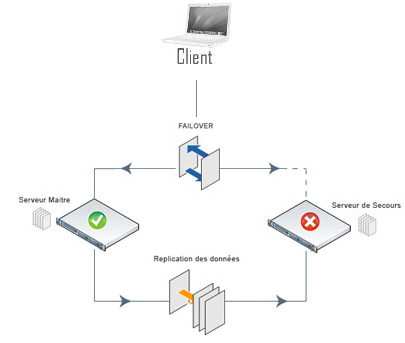
\includegraphics[scale=0.9]{Images/SchemaCluster.png}
	\caption{Cluster, serveur maître et esclave directement connectés}
	\label{SchemaCluster}
\end{figure}

%\begin{figure}[htbp]
%	\centering
%	\begin{tikzpicture}
%	    % Styles :
%		\tikzstyle{titre}=[rectangle,draw,fill=white,text=black]
%		\tikzstyle{symbole}=[rectangle,text=black, scale=4]
%		\tikzstyle{serveurloc1}=[rectangle,draw,fill=blue!50,text=white, minimum height=2cm]
%		\tikzstyle{serveurloc2}=[rectangle,draw,fill=yellow!50,text=black, minimum height=2cm]
%		\tikzstyle{serveurcentral}=[rectangle,draw,fill=violet!50,text=black, minimum height=2cm]
%		
%		% #### CADRE VERT :
%		% Fond :
%		\draw[fill=green!10] (0,6) rectangle (16, 11);
%		\draw[fill=red!10] (2,11) rectangle (11, 6);
%		% Titres :
%		\node[titre] at (6.50,7.00) {Serveur local};
%		% Serveurs :
%		\node[serveurloc1] at (4.00,8.50) {Serveur maître};
%		\node[serveurloc2] at (9.00,8.50) {Serveur esclave};
%		\node[serveurcentral] at (14.00,8.50) {Serveur central};
%		% Traits :
%		\draw[line width=2pt] (1.5, 8.5) -- (2, 8.5);
%		\draw[line width=2pt] (5.5, 8.5) -- (7.5, 8.5);
%		\draw[line width=2pt] (11, 8.5) -- (12.5, 8.5);
%		% Utilisateurs :
%		\umlactor[x=1.00, y=8.50]{Utilisateur}
%	\end{tikzpicture}
%
%\caption{Cluster, serveur maître et esclave directement connectés}
%	\label{explicationcodeco}
%\end{figure}

Le serveur de secours est en \emph{hot standby}, c'est-à-dire qu'il reste allumé en mode passif, attendant que des requêtes clients soient reçues (requêtes qui sont envoyées au maître tant que ce dernier est actif).

\paragraph{Fail-over}
Dans le cadre d'une architecture serveur haute disponibilité, le \emph{fail-over} permet une reprise automatique inférieure à une minute sur le serveur de secours en cas de défaillance du serveur maître. Le \emph{fail-over} est donc la capacité d'un équipement à basculer automatiquement vers un chemin réseau redondant ou en veille.
Cette solution est préconisée sur les serveurs ou les architectures serveurs qui nécessitent une disponibilité permanente et un haut niveau de connectivité.
\\
Il existe deux utilisations du protocole \emph{fail-over}~:
\begin{itemize}
	\item mode statique~: chaque client est configuré pour basculer sur une URI précise si la standard ne répond plus~;
	\item mode dynamique~: le maître fournit dynamiquement l'URI de l'esclave aux clients qui peuvent la mettre à jour.
\end{itemize}
Le mode retenu est le mode statique, où chaque client a sa configuration et la conserve, aucune configuration spécifique n'est donc nécessaire pour le maître, et il faut simplement configurer sur l'esclave la connection avec le maître.

\paragraph{Réplication des bases de données en temps réel}
Les écritures sur le serveur maître sont répliquées en temps réel sur le serveur de secours, ne ralentissent pas le serveur maître et permettent de minimiser les pertes de données.
La réplication se fait par recopie des journaux de transactions entre le maître et l'esclave.
\\
Le mode de synchronisation choisi est le mode synchrone~: une transaction émise par un client n'est validée que si l'écriture sur le maître ainsi que la synchronisation avec le serveur de secours sont validées.
Ceci permet de s'assurer de la bonne duplication des données sur les deux serveurs. 

\paragraph{Limitations}
Seul un esclave à la fois peut être connecté au maître.
Un maître hors ligne ne peut être réintroduit qu'à froid.
Répliquer les données de l'esclave vers le maître une fois ce dernier remonté n'est pas automatique, cela nécessite une intervention manuelle.

\paragraph{Logiciel}
Apache Active MQ est un agent de messages open source, écrit en Java et associé avec un client Java Message Service.
Cette suite prend en charge divers protocoles de transport et précisément le protocole de fail-over qui permet de configurer les clients afin qu'ils basculent sur le serveur esclave en cas de non réponse du maître. 
Il permet aussi de charger les différentes configurations (clients, maître et esclave) conservées dans des fichiers XML. 

\subsection{Sauvegarde en dur}
Une deuxième solution peut être mise en œuvre de manière complémentaire au \emph{cluster} afin de mieux respecter la contrainte concernant l'intégrité des données.
Un support mobile de stockage est utilisé afin de directement sauvegarder le contenu des serveurs.
Le support peut être un disque dur, une clé USB, une carte mémoire...
Cette sauvegarde devra être effectuée toutes les six heures afin de permettre de remonter les données en cas de panne des deux serveurs.  
